\chapter{Implementation\label{chap:implementation}}

To answer the Research Question proposed on page~\pageref{section:research-question}, this project implements the reviewer recommender system so that they can be evaluated later in Chapter~\ref{chap:evaluation}. The implementation performed in this project can be broken down into the following items:
\begin{itemize}
    \item Data collection over many different sources of data
    \item Implementation of a rule based recommender
    \item Implementation of a neural network based recommender
    \item Supporting code for both recommenders
\end{itemize}

Data collection was implemented first as this was needed for the other items to be possible. Supporting code was written for both recommender implementations that allowed common interfaces to the implementations, result classes returned by the recommender implementations and methods for collating the collected data into a format understandable by the recommender implementations. Two implementations of the recommender implementations are built so that they can be compared against each other. Furthermore, the rule based implementation was used as a trial run for the neural network implementation which allowed us to find many issues with the data collected and fix them before this required re-training neural network models.

To make the code easier to debug, we used Python's in-built logging library\footnote{\url{https://docs.python.org/3/library/logging.html}. Accessed 12 May 2023} that allowed us to send information to file instead of printing it to the console. The logs were placed in a centralised location, but are not included in the project submission as they are too large and verbose.

\section{Data Collection\label{section:data-collection-implementation}}

Data needs to be collected in this project so that the implementations of the reviewer recommender system can use this data to make recommendations. Therefore the data collection, while not directly answering the research question, is an important and unavoidable step towards answering it.

We first tried to get the data set downloaded in one go by requesting access to the database of the system. Andre Klapper was contacted to provide this data, however, he was unable to provide the raw data in a dump as it had non-public data mixed into it. As such the data had to be collected using APIs that had access to this information. This did make data collection more complicated but did not end up hindering the project too much.

To collect the data we used several sources. These included:
\begin{itemize}
    \item Bitergia Analytics elastic search API.
    \item Gerrit REST API.
    \item The git repositories themselves which are downloaded from the Gerrit system by cloning the repository onto the author's PC.
\end{itemize}

Without these sources of data, the project would have not been possible to achieve. This is because manually scraping the data by loading the web page and parsing it to extract the data would have been highly inefficient, extremely prone to bugs and likely overuse the resources provided by the Gerrit system.

For example, trying to parse the information about a change using the page as shown below in Figure~\ref{fig:checkuser-example-change-for-scraping-example} would require a lot of inspection surrounding the HTML classes assigned to each area that has data to be scraped. In this example page, there are at least 8 different places where data would be parsed from. If the data was collected for the entire repository and all its changes, this would mean sending out thousands of HTTP GET requests instead of making one request to the API for the data.

\begin{figure}[h]
    \centering
    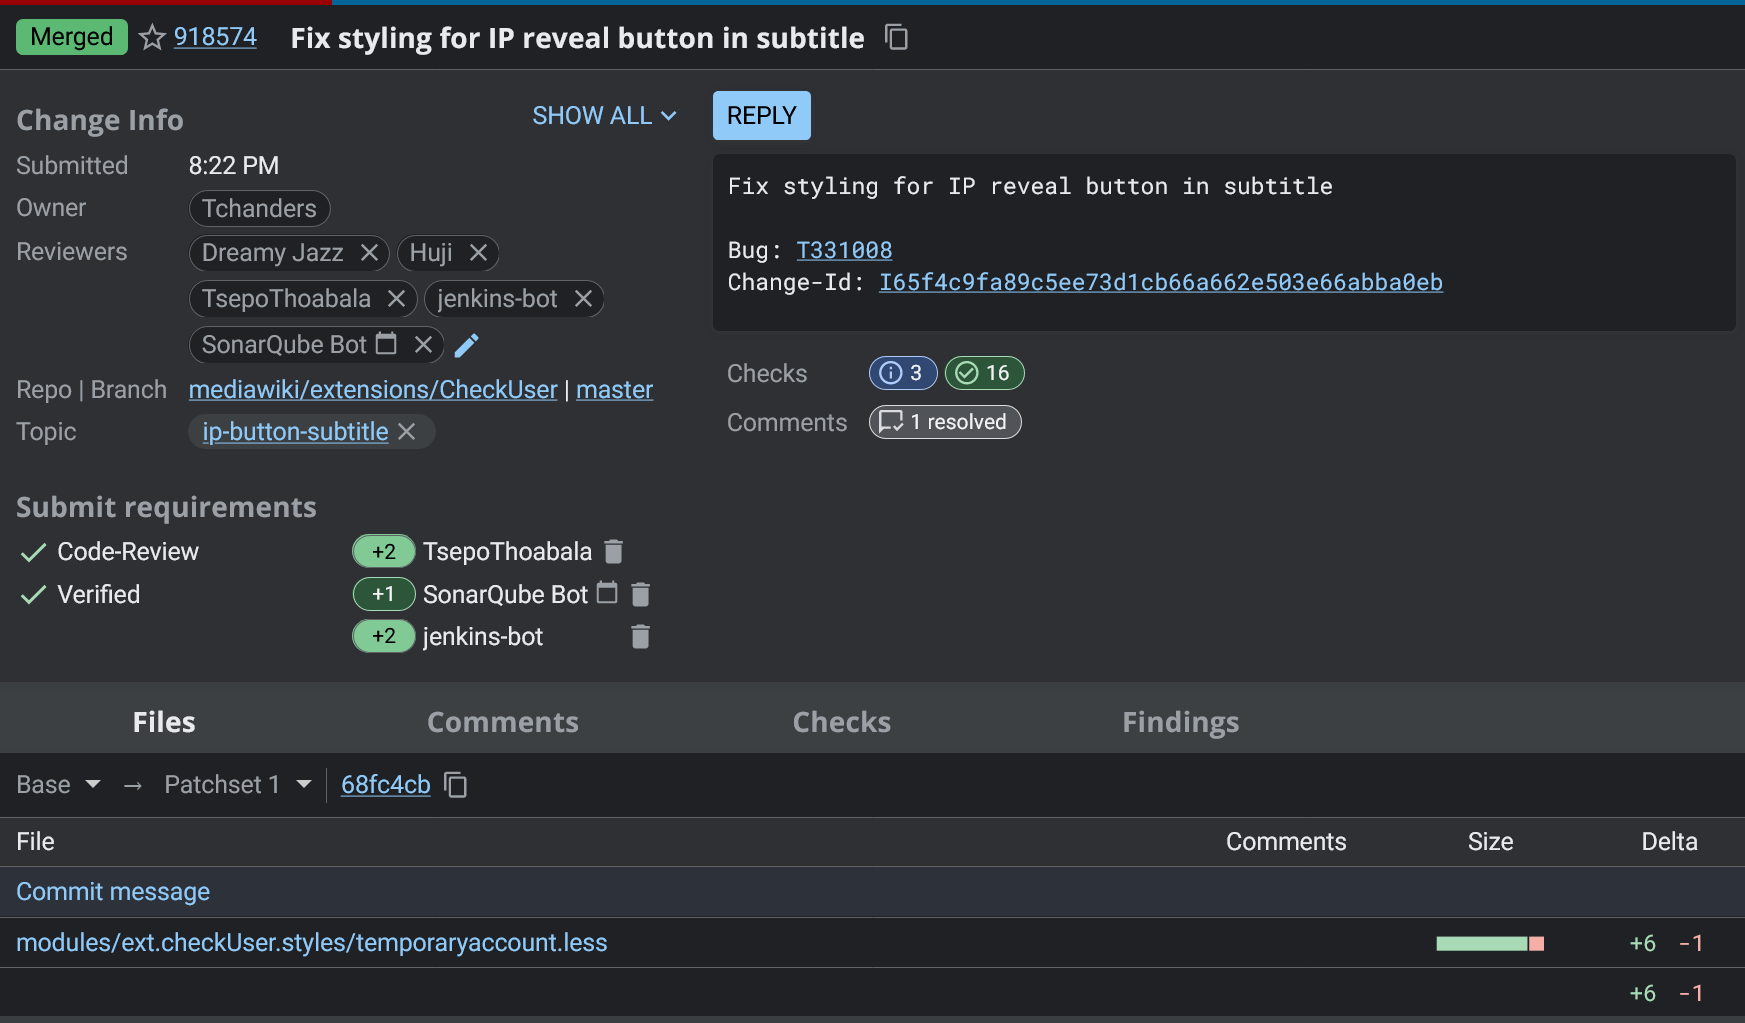
\includegraphics[scale=0.23]{images/checkuser-example-change-information-page.png}
    \caption{Page for example merged change in the CheckUser extension.}
    \label{fig:checkuser-example-change-for-scraping-example}
\end{figure}

The Gerrit REST API provides everything that can be got from the change page as shown in the example change above. When the data needs to be grouped by user and/or repository sometimes using the Gerrit API wouldn't work as well as using the Bitergia Analytics system.

To access the data in the Gerrit REST API, the MediaWiki Gerrit installation required that the request provide authentication. This is done in this project by providing the Authorization header with an HTTP password \citep{gerrit:authentication}. This HTTP password was generated using the user account owned by the author, which also had rights to approve code over every repository starting with the prefix ``mediawiki''. It was unclear whether the requirement to authenticate to use the REST API also required that the user account being used has the right to approve code.

While the Gerrit API requires authentication to be used, all the data provided by the Gerrit API that was collected is publicly available in a different format through the Bitergia Analytics site and by viewing changes on the Gerrit site. As such there are no privacy concerns that come from making available the data collected from the Gerrit API.

The Bitergia Analytics Elasticsearch API did not require any authentication, though the documentation on MediaWiki's website specified that you needed an account to get access \citep{mediawiki:community-metrics}. However, this does not seem to be the case and we were able to make requests to the API. Private data seemed to be hidden in testing using the API, so privacy concerns on using this data are also very small to none. The data collected from this API is also available from the Gerrit system, but the way the results are grouped makes the system more suitable when collecting data that is generalised into groups.

The Bitergia Analytics API uses Elasticsearch which is a ``distributed search and analytics engine'' \citep{elastic:elastic-search-intro}. Queries to the API in this project make GET requests to the endpoint and specify the parameters for the query in the request body as JSON.

To make the API requests using Python, we investigated using preexisting packages such as the package ``elasticsearch''\footnote{\url{https://pypi.org/project/elasticsearch/}. Accessed 12 May 2023}. However, these packages did not provide what was needed to make the requests. As such a custom builder for the elastic search requests was created that provided the features that were needed.

The queries used to generate the data were based on queries used panels shown on the MediaWiki Bitergia Analytics site. Each panel could be easily inspected to find the API request along with the JSON request body used. This was adapted and then rewritten using the elastic search query builder created for this project. An example page that had some of the panels inspected for this project is the `Gerrit Approvals' page\footnote{\url{https://wikimedia.biterg.io/app/kibana\#/dashboard/95487340-6762-11e9-a198-67126215b112?\_g=()}. Accessed 14 May 2023.} that details approval votes statistics, including approval voters per user.

One downside with collecting data from both the Gerrit API and Bitergia Analytics API is that the name used to identify the same user was sometimes different between the sources. To help address this the Gerrit API requests were always asked for detailed account information which provided other names, account ID and email address associated with each user that is shown in the results \citep{mediawiki-gerrit:changes-rest-api-detailed-accounts}. However, this is not foolproof and the reviewer recommender implementations described later in this chapter will perform some anti-duplication techniques to help address this problem.

The repositories were easily cloned from the Gerrit system. For the main data collection, the repositories were bare-cloned, which means that the files in the repository were not created and instead only the information about the repository (including commit histories) are available. This is all that was needed for the data collection for the implementation, however, for the evaluation in Chapter~\ref{chap:evaluation} some of the repositories were normally cloned to count the number of files in the repository. Using a bare-cloned repository made the folder size for each repository smaller, which significantly reduced the size of this data.

The table in Table~\ref{table:data-collected-stats} the data collected is detailed along with some statistics and where it was collected from. In Table~\ref{table:data-collected-grouping} how the data is grouped is shown.
\begin{table}[H]
    \centering
    \begin{tabular}{@{}c c c c@{}}
    \hline
    \textbf{Name} & \textbf{Data points} & \textbf{File(s) size} & \textbf{Source} \\
      \hline
      Repositories & {\raise.17ex\hbox{$\scriptstyle\sim$}}1,400 & 0.3 MB & Gerrit API \\
      Users with rights to approve changes & {\raise.17ex\hbox{$\scriptstyle\sim$}}1,600 & 1 MB & Gerrit API\\
    Comment counts & {\raise.17ex\hbox{$\scriptstyle\sim$}}50,000 & 1.8 MB & Bitergia Analytics API \\
    Code review vote counts & {\raise.17ex\hbox{$\scriptstyle\sim$}}250,000 & 9.2 MB & Bitergia Analytics API \\
    Git blame & N/A & 1.93 GB & Gerrit git repositories \\
    All changes from defined periods & {\raise.17ex\hbox{$\scriptstyle\sim$}}64,000 & 201 MB & Gerrit API\\
    \hline
    \end{tabular}
    \caption{The data collected for this project and associated statistics.}
    \label{table:data-collected-stats}
\end{table}

\begin{table}[H]
    \centering
    \begin{tabular}{@{}c c c c c c c@{}}
    \hline
    \textbf{Name} & \multicolumn{3}{c}{\textbf{Grouped by}} \\
    & {Repository} & {Author} & {Time period} & {File} \\
      \hline
      Repositories & & & & \\
      Users with rights to approve changes & \checkmark & & & \\
      Comment counts & \checkmark & \checkmark & \checkmark & \\
      Code review vote counts & \checkmark & \checkmark & \checkmark & \\
      Git blame & \checkmark & & & \checkmark \\
      All changes from defined periods & \checkmark & & \checkmark & \\
      \hline
    \end{tabular}
    \caption{The data collected for this project and how it was grouped.}
    \label{table:data-collected-grouping}
\end{table}

The data that was first collected is the repositories. This was done first so that data which is grouped by repository could be collected.

The repositories collected are those hosted on the MediaWiki Gerrit system with the prefix ``mediawiki/''. Other repositories exist on the MediaWiki Gerrit system without this prefix, but they don't relate to the MediaWiki project as a whole. For example, the repository ``operations/mediawiki-config'' is a repository for the configuration settings used on the wikis hosted by the Wikimedia Foundation (such as Wikipedia) \citepmediawiki{mediawiki:operations-mediawiki-config-readme}. This repository is less similar to a repository for an extension to MediaWiki and in some cases has a different accepted practice for merging. For example, in some repositories, the author of the change performs the approval vote after another user with the right to approve gives a ``+1'' vote.

For the collection of the users with rights to approve changes, the members of each group that has the rights to approve code are collated into one list. The code that does this is roughly equivalent to the pseudo-code in Algorithm~\ref{alg:data-collection-members-of-repositories}. This data was collected as it was important to know if the recommendations produced contained a good proportion of users who could approve the change. It is important to have this mix of users who can approve and users who can vote so that people are recommended who can merge the change while also recommending active users who can provide feedback before an approver sees the change.

\SetKwProg{Fn}{Function}{}{}
\begin{algorithm}[H]
	\Fn{get\_members\_of\_repositories (repository)}{
		$groups \gets groups\_with\_access\_to\_repository$ $(repository)$\;
            $members\_of\_repository = set()$\;
            \ForEach{$\{group\} \in groups$}{
                $members\_of\_repository \gets members\_of\_repository \cup members\_of\_group$ $(group)$\;
            }
            $parent\_repository \gets get\_parent\_repository$ $(repository)$\;
            \If{$parent\_repository$ $exists$}{
                $members\_of\_repository \gets members\_of\_repository \cup get\_members\_of\_repositories$ $(parent\_repository)$\;
            }
		\Return $members\_of\_repository$\;
	}
	\caption%[An algorithm with an optional, shorter caption]%
	{\label{alg:data-collection-members-of-repositories}Data collection for members of repositories.}
\end{algorithm}

The number of comments per user per repository was collected as it was seen as an indicator of activity that also considered users who could not approve changes but otherwise provide useful feedback. The number of comments was collected over four different time periods which are: all time, last year, last three months and last month.

The number of code review votes was also collected in a similar way to the number of comments. They were grouped by code review value (e.g. ``+1'') per user per repository. This was collected as we hypothesised that having more votes on a repository is an indication of being more active on the repository.

Both the number of comments and the number of code review votes were converted from the raw counts into percentages. This was done so that the comment and code review vote counts for each user were stored as a proportion of the total count for all users. This means the values are between 1 and 0 and should also add up to 1.

The authors and committers of changes that modified files were generated using git-blame. git-blame is a tool that returns ``what revision and author last modified each line of a file'' \citep{git:git-blame}. This data cannot be collated by file in advance because:
\begin{itemize}
    \item The comparison is performed against the parent commit for the change (or branch if the parent commit doesn't exist on the local clone). This can be any commit (or branch) for the repository and is only known when the change is provided to make recommendations
    \item The files modified by the change could be any combination of files that exist in a repository (later on page~\pageref{paragraph:mediawiki-core-being-large-in-file-count} we discuss how this number can be many hundreds of thousands for ``mediawiki/core''). Collating all data for all files into a JSON file would create a highly unmanageable dataset.
\end{itemize}

The git-blame tool is therefore run at run time and the data is collated when making the recommendations. To limit the effect that this has on the run time, files that exceed a set size are skipped when collating this data. The code that collects this data from git-blame is roughly equivalent to the pseudo-code shown in Algorithm~\ref{alg:git-blame-dataset}.

\begin{algorithm}[H]
	\Fn{get\_git\_blame\_data (repository, files, parent\_commit, branch)}{
            $git\_repo \gets get\_bare\_cloned\_repo$ $(repository)$\;
            \eIf{$parent\_commit \in git\_repo$}{
                $git\_repo \gets update\_git\_head\_to\_commit$ $(repository, parent\_commit)$\;
            }{
                $git\_repo \gets update\_git\_head\_to\_branch$ $(repository, branch)$\;
            }
            $valid\_time\_periods \gets \{last\_month, last\_three\_months, last\_year, all\_time\}$\;
            $author\_lines\_count \gets \{\}$\;
            $committers\_lines\_count \gets \{\}$\;
            \ForEach{$file \in files$}{
                $git\_blame\_entries \gets get\_git\_blame\_entries\_for\_file$ $(git\_repo, file)$\;
                \ForEach{$blame\_entry \in git\_blame\_entries$}{
                    $line\_counts \gets get\_line\_counts\_for\_blame\_entry$ $(blame\_entry)$\;
                    $commited\_date \gets get\_associated\_date\_with\_blame\_entry$ $(blame\_entry)$\;
                    $author \gets get\_author\_for\_blame\_entry$ $(blame\_entry)$\;
                    $committer \gets get\_committer\_for\_blame\_entry$ $(blame\_entry)$\;
                    \ForEach{$time\_period \in valid\_time\_periods$}{
                        \If{$(time\_period~starts~before~commited\_date) \lor (time\_period = all\_time)$}{
                            \If{$time\_period \not \in author\_lines\_count[repository][author]$}{
                                $author\_lines\_count[repository][author]\newline[time\_period] = 0$\;
                            }
                            $author\_lines\_count[repository][author]\newline[time\_period]~$+=$~line\_counts$\;
                            \If{$time\_period \not \in committers\_lines\_count[repository][committer]$}{
                                $committers\_lines\_count[repository][committer]\newline[time\_period] = 0$\;
                            }
                            $committers\_lines\_count[repository][committer]\newline[time\_period]~$+=$~line\_counts$\;
                        }
                    }
                }
            }
            \Return $(author\_lines\_count, committers\_lines\_count)$\;
	}
	\caption%[An algorithm with an optional, shorter caption]%
	{\label{alg:git-blame-dataset}Data collection of git-blame info}
\end{algorithm}
\hspace{1cm}

Previous research that implemented reviewer recommender systems used git-blame data to make recommendations and we hypothesised that a user who authored or committed changes to a file has a better understanding of the file than the average user. As such collecting this data was a clear choice.

Finally, a training and testing data-set of merged, open and abandoned changes was collected for each repository. This was done to allow evaluation of the reviewer recommender implementations offline as the tool could be given the downloaded change information instead of requesting that from the Gerrit API. The method to collect this is roughly detailed by the pseudo-code in Algorithm~\ref{alg:data-collection-dataset}.

\begin{algorithm}[H]
	\Fn{get\_test\_and\_training\_data\_set (repository)}{
            $valid\_time\_periods \gets \{last\_month, last\_three\_months, last\_year, all\_time\}$\;
            \ForEach{$time\_period \in valid\_time\_periods$}{
                $changes\_from\_time\_period \gets get\_changes\_from\_time\_period\_for\_repository$ $(repository, time\_period)$\;
                $merged\_changes\_from\_time\_period \gets filter\_for\_merged\_changes$ $(changes\_from\_time\_period)$\;
                \If{($|merged\_changes\_from\_time\_period| \geq 10) \lor (time\_period = all\_time)$}{
                    \Return $changes\_from\_time\_period$\;
                }
            }
	}
	\caption%[An algorithm with an optional, shorter caption]%
	{\label{alg:data-collection-dataset}Data collection of the testing and training data set.}
\end{algorithm}

\label{para:limited-to-ten-merged-changes}The changes that were collected come from time periods specific to each repository such that the smallest time period is used that returns at least 10 merged changes. This is done to limit the amount of data that was collected as repositories such as mediawiki/core has many changes made which would make selecting changes from all time or even just the last year very data-intensive to generate. Furthermore, where possible the changes collected were ideally newer than older as the relationships between the data features and the changes collected could have changed if the change is too old. For example, a user who was very active in reviewing changes but stopped 6 months ago could be recommended and seen as a good recommendation in the evaluation performed in Chapter~\ref{chap:evaluation}.

\label{para:information-in-each-change-for-testing-data-set}Each change in the training and testing data-set contained the following information:
\begin{enumerate}
    \item The owner of the change
    \item The Change-ID for the change
    \item The branch of the change
    \item Any associated tracking IDs for the change
    \item The files modified in the change
    \item The parent change(s) (otherwise known as a parent commit(s)).
    \item The total comment count on the change
    \item The number of unresolved comments on the change
    \item The code review votes given to the change
    \item The users added as reviewers to the change
\end{enumerate}

Items 4, 7, 8 and 10 were not used in the implementation of the recommenders as they were deemed not useful in making recommendations after the data was collected. However, items 7, 8 and 10 are seen as potentially useful for evaluation of the implementations if they were used live on the Gerrit system. This means that this data, while not used in this project, may have uses for future research. For example, the data about the reviewers on the change could be used to suggest that a recommendation was accepted by looking for when the reviewer was added and comparing it to when the recommendations were made.

Using a JSON file to store the collected training and testing data was not immediately obvious. This is because when using the standard JSON library the entire training and testing data set is loaded into memory. Considering this is about 200 MB in size when saved to the disk, keeping this in memory when performing training of a model could make a noticeable impact on running time. The use of an SQLite database was considered as Python supports using SQLite, SQLite supports holding JSON data in tables, and it would allow getting data one repository at a time. However, the file size of the database was three times as large as the training and testing data-set. An alternative to the JSON library was found called `ijson'\footnote{\url{https://pypi.org/project/ijson/}. Accessed 12 May 2023.} which allows loading the JSON file iteratively, and was used to load the data for use in the reviewer implementations.

The training and test data set was collected at least 4 times as the algorithm used to collect and filter the data had bugs or was missing data that was later determined to be needed. Because the data being collected was so large in size, the script would take around a day to complete. A large proportion of this time was waiting for HTTP requests but also included throttling the requests to not overload the servers.

\label{para:data-inspected-but-not-used}Some data was inspected but not used for the project. One of these data sources is the Code maintainers list\footnote{\url{https://www.mediawiki.org/w/index.php?title=Developers/Maintainers&oldid=5899598}. Accessed 2 May 2023} which is a list of steward teams and maintainers of code that is deployed on WMF wikis. This was not used as the data provided by it was not comprehensive for all repositories and when implementing the rule based recommender (as discussed in section~\ref{section:rule-based-implementation}) the data was deemed as not useful.

\section{Recommender Implementation}

Two implementations, a rule based and a neural network based implementation, have been built. Work started on these implementations once the data collection was mostly complete. Both implementations meet the functional requirements specified in section~\ref{section:recommender-requirements}. The non-functional requirements are all met by the rule based recommender as discussed here and later in Chapter~\ref{chap:evaluation}. The neural network recommender implementation mostly meets the non-functional requirements, but doesn't meet the first non-functional requirement as well as the rule based does. This is discussed further in section~\ref{section:rule-based-against-neural-network}.

After data collection was mostly complete, work started on building the recommender implementations that would use the collected data to make recommendations.  Both implementations discussed here meet the functional requirements discussed for the recommender implementations in section~\ref{section:recommender-requirements} though the second implementation doesn't meet the non-functional requirements as well as it could do.

\subsection{Supporting Code\label{section:supporting-code}}

Both implementations of the reviewer recommender system use similar `supporting code' to make their recommendations. This includes code that:
\begin{itemize}
    \item Reads and prepares the data collected for the project in a format that can be understood by the recommender implementations
    \item Provides methods that can be used to ask for recommendations that are independent of the implementation.
    \item Provides common result classes that allow callers to interact with the same methods independent of the implementation they use
    \item Provides anti-duplication techniques to the result data
\end{itemize}

While the supporting code makes it possible to use the system only with knowledge of the name of the implementation, it is not necessarily designed to make the implementations work out of the box on other open-source projects.

When loading the data from a file and repeated calls to the same function for the same output were expected, we used the lru\_cache decorator\footnote{\url{https://docs.python.org/3/library/functools.html\#functools.lru\_cache}. Accessed 12 May 2023.} from Python's inbuilt functools library. This memoises the function that the decorator is attached to, which means that if a previous call used the same arguments for the function the result returned for that call would be returned.

The git-blame and result classes were partly covered by tests built using Python's unittest library\footnote{\url{https://docs.python.org/3/library/unittest.html}. Accessed 13 May 2023.}. Although the code was not written using test-driven-development, the need for tests became apparent as the project proceeded. Bugs were found that caused re-runs of scripts which take a long time to run, such as the training of the neural network implementation as discussed on page~\ref{para:neural-network-length-of-training-considerations}. The decision to not write a lot of tests was made because other areas of the project were prioritised over writing tests. If there was more time to work on this project, we would consider writing tests for the code.

\label{para:de-duplication-supporting-code}To ensure that recommendations are not duplicated, methods to convert usernames and emails to their ``index form'' exist and are used throughout. For usernames this means stripping whitespace, converting to lowercase, and replacing ``-'' and ``\_'' characters with a space. For email addresses, this means stripping whitespace and converting to lowercase. If two names or two emails are the same when converted to index form, they are considered the same user and therefore their entries are merged. Where this method did not work appropriately, a map of usernames to email addresses was globally defined that would help remove duplication if the duplicated entries used an email for one and a name for the other.

A result class was implemented that allowed easy inspection of the results without the need to necessarily know which implementation the results came from. The class which is named $Recommendations$ provides methods to get the top N users, find recommended users by their username or email and merge entries if they are duplicates. The $Recommendations$ class holds references to $RecommendedReviewer$ classes that hold information about a recommended reviewer. The classes are linked together in a two-way relationship with the link from the recommended reviewer being implemented using Python's weakref module\footnote{\url{https://docs.python.org/3/library/weakref.html}. Accessed 13 May 2023.}.

\subsection{Rule Based Recommender\label{section:rule-based-implementation}}

The first recommender implementation built was the rule based recommender system. This system uses pre-determined weights on the collected data to make recommendations. This was built before the neural network implementation as modifying the data was used to make the recommendations would not require re-training if modifications were needed. For example, data mentioned in the data collection section on page~\pageref{para:data-inspected-but-not-used} that was excluded was excluded based on implementing the rule based recommender. If this was excluded after the model had been built it would require re-training the models which is a lengthy process as described on page~\ref{para:neural-network-length-of-training-considerations}.

As such getting the rule based recommender working, even if performed poorly, was the next biggest priority after the data collection with respect to the programming in this project. Getting it working would also mean that there is an implementation that works in case the neural network recommender system failed and couldn't be fixed before the project was finished.

The rule based recommender can produce recommendations using:
\begin{itemize}
    \item A Change-ID for a change on the MediaWiki Gerrit system (requiring the branch and repository if the change with the Change-ID exists on multiple repositories/branches)
    \item The change info that would be downloaded by the system if only the Change-ID was passed.
\end{itemize}

The change info that is needed is provided by the training and testing data set, which means that the recommender can be evaluated using changes from that data set.

The pseudo-code in Algorithm~\ref{alg:rule-based} gives a rough idea of what the rule based recommendation does to produce recommendations when given the change information. If given the Change-ID the change information is downloaded from the Gerrit API and then passed to the same code. The rule based recommendation approach is also detailed in Figure~\ref{fig:rule-based-flowchart} as a flowchart.

\begin{figure}[h]
    \centering
    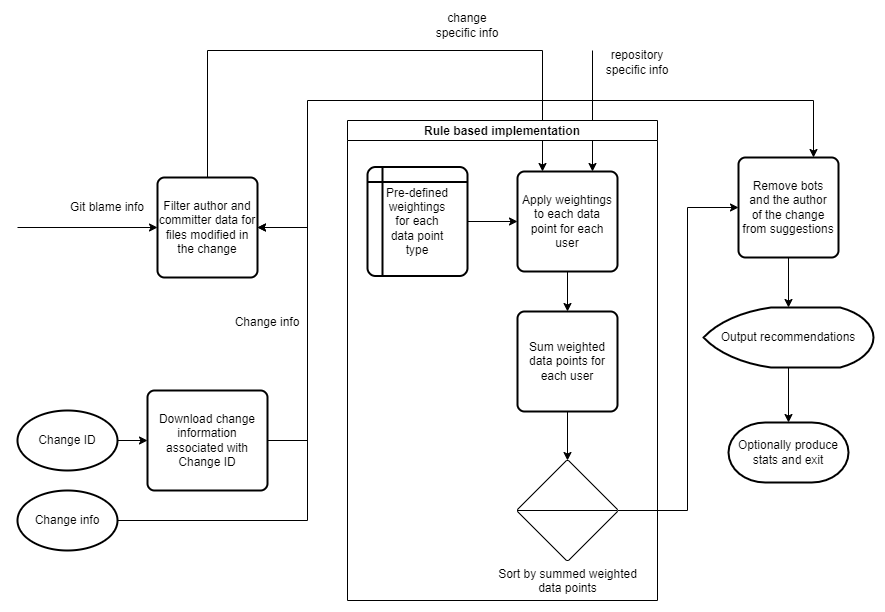
\includegraphics[scale=0.45]{images/rule-based-flowchart.png}
    \caption{Flowchart describing the process used by the rule based implementation.}
    \label{fig:rule-based-flowchart}
\end{figure}

\begin{algorithm}[h]
	\Fn{rule\_based\_recommender (change\_info)}{
            $recommendations \gets get\_recommendations\_result\_class()$\;
            $weighings \gets get\_weighings()$\;
		$recommendations.exclude\_user(change\_info[$\enquote{$owner$}$])$\;
            $repository \gets change\_info[$\enquote{$repository$}$]$\;
            $files\_in\_change \gets get\_files\_in\_change$ $(change\_info)$\;
            $parent\_change \gets change\_info[$\enquote{$change\_info$}$]$\;
            $branch \gets change\_info[$\enquote{$branch$}$]$\;
            $author\_lines\_count, committers\_lines\_count \gets get\_git\_blame\_data$ $(repository, files\_in\_change, parent\_change, branch)$\;
            $members\_of\_repositories \gets get\_members\_of\_repositories$ $(repository)$\;
            \ForEach{$user \in members\_of\_repositories$}{
                $reviewer \gets recommendations.add\_recommendation$ $(user)$\;
                $reviewer.has\_rights\_to\_merge = True$
            }
            \ForEach{$author, lines\_count\_by\_period \in author\_lines\_count$}{
                $reviewer \gets recommendations.add\_recommendation$ $(author)$\;
                \ForEach{$time\_period, lines\_count \in lines\_count\_by\_period$}{
                    $reviewer.add\_score$ $(lines\_count, weighings[$\enquote{$author\_lines\_count$}$][time\_period])$\;
                }
            }
            \ForEach{$committer, lines\_count\_by\_period \in committers\_lines\_count$}{
                $reviewer \gets recommendations.add\_recommendation$ $(committer)$\;
                \ForEach{$time\_period, lines\_count \in lines\_count\_by\_period$}{
                    $reviewer.add\_score$ $(lines\_count, weighings[$\enquote{$committer\_lines\_count$}$][time\_period])$\;
                }
            }
            $vote\_data \gets get\_vote\_data\_for\_repository$ $(repository)$\;
            \ForEach{$user, vote\_counts\_for\_user \in vote\_data$}{
                $reviewer \gets recommendations.add\_recommendation$ $(user)$\;
                \ForEach{$vote\_type, vote\_count \in vote\_counts\_for\_user$}{
                    $reviewer.add\_score$ $(vote\_count, weighings[$\enquote{$votes$}$][vote\_type])$\;
                }
            }
            $comment\_data \gets get\_comment\_data\_for\_repository$ $(repository)$\;
            \ForEach{$user, comment\_counts\_for\_user \in comment\_data$}{
                $reviewer \gets recommendations.add\_recommendation$ $(user)$\;
                \ForEach{$comment\_type, comment\_count \in comment\_counts\_for\_user$}{
                    $reviewer.add\_score$ $(comment\_count, weighings[$\enquote{$comments$}$][comment\_type])$\;
                }
            }
		\Return $recommendations$\;
	}
	\caption%[An algorithm with an optional, shorter caption]%
	{\label{alg:rule-based}Rule based recommender}
\end{algorithm}

The weightings associated with the rule based recommender were stored in a JSON file. This was done to allow inspection and modification to the weightings using any text editor. The weightings were applied using the $add\_score$ method that multiplies the weighting against the value for the data point and then adds the result to the existing score.

Through the implementation of this rule based method, the associated weightings were modified 2 times to make the recommendations better. However, further modification could be done to make the weightings better.

\subsection{Neural Network Recommender\label{section:neural-network-recommender-implementation}}

Starting the machine learning implementation was much more complicated. This is because a process of finding the correct technique to use to recommend reviewers was required. Research into the options found at least 5 other ways to implement it using machine learning, including using LamdaRank\footnote{\url{https://www.microsoft.com/en-us/research/wp-content/uploads/2016/02/MSR-TR-2010-82.pdf}. Accessed 1 May 2023.} and a convolutional neural network. However, the decision was made to use Mutli-Layer Perception (MLP) classifier as the neural network method for this implementation.

MLP is a type of ``neural network that learns the relationship between linear and non-linear data'' \citep{towardsdatascience:mlp-classifier}. It has input and output layers that are combined together using a number of hidden layers, where each layer ``is feeding the next one with the result of their computation'' which makes it a feedforward algorithm \citep{towardsdatascience:mlp-classifier}. The MLP when learning uses backpropagation to ``iteratively adjust the weights in the network, with the goal of minimizing the cost function'' \citep{towardsdatascience:mlp-classifier}. This means that this method should be a good method to use.

For this implementation in Python, sklearn's MLPClassifier implementation is used\footnote{\def\UrlBreaks{\do\/\do-\do.}\url{https://scikit-learn.org/stable/modules/generated/sklearn.neural\_network.MLPClassifier.html}. Accessed 12 May 2023.\def\UrlBreaks{\do\/\do-}} as the model. sklearn, otherwise known as `scikit-learn', is an open-source machine learning library for Python. It provides a good MLP classifier implementation and also provides many other methods to prepare the data and test the model.

This implementation used many MLP classifier models that were trained and tested using different parts of the training and testing data set. Each model that was trained came as a pair of a model that predicted if a user would approve a change and then a model to predict if a user would vote on a change. Table~\ref{table:mlp-model-types} details the different types of models as well as what changes were used to train and test the model pairs.

\begin{table}[H]
\begin{center}
\begin{tabular}{@{}c c c c c@{}} 
\hline
\textbf{Model type} & \multicolumn{4}{c}{\textbf{Changes used for training and testing}} \\
 & All changes & \multicolumn{3}{c}{Repository specific} \\
& & Merged changes & Open changes & Abandoned changes \\
\hline
Generic & \checkmark & & & \\
Repo-specific &  & \checkmark & \checkmark & \checkmark \\
Merged & & \checkmark & & \\
Open & & & \checkmark & \\
Merged & & & & \checkmark \\
\hline
\end{tabular}
\end{center}
\caption{
\label{table:mlp-model-types}The different types of model pairs and what data was used to train them.}
\end{table}

The ``Generic'' model type is given all the changes that are used for training and is used to make predictions on any repository. The ``Repo-specific'' model type is used to make predictions on changes for the repository it is trained on and is passed all the training data for the repository it is assigned. The ``Open'', ``Merged'' and ``Abandoned'' model types are models that are only trained on open, merged or abandoned changes respectively for a particular repository. These three model types can only be used to predict the reviewers for changes with the associated status on the associated repository.

The generic model type provides advantages as it is not subject to the cold start problem if new repositories are created. However, the number of repositories being evaluated may cause the data to be too sparse to produce accurate recommendations for every repository. This is discussed in further detail in Chapter~\ref{chap:evaluation}.

\label{para:neural-network-length-of-training-considerations}If trained for all repositories, the generic type would have one model pair and every other type would have {\raise.17ex\hbox{$\scriptstyle\sim$}}1,400 model pairs. For the evaluation in Chapter~\ref{chap:evaluation}, not all of the repositories were used for training and testing as the time to generate the {\raise.17ex\hbox{$\scriptstyle\sim$}}4201 model pairs (8402 models in total) would take too long to complete before the project completion date. This was because the final run of the training for the neural network implementation was only about a week before the project's conclusion. This was because there were a number of bugs and issues that necessitated the models being re-trained 4 times.

We chose this many pairs to make it possible to compare the evaluation scores for each model type and then make recommendations using the best-performing model types. It also reduced the chance that a model failing would prevent the implementation from working as other models could be selected instead.

\hspace{0.25cm}
\subsubsection{Training\label{section:rule-based-implementation-training}}

Each model was trained using the appropriate part of the testing and training data-set of changes. A high-level description of this process is shown in Figure~\ref{fig:neural-network-training-flowchart} as a flowchart. This is done instead of detailing the pseudo-code as the flowchart is easier to understand.

\begin{figure}[h]
    \centering
    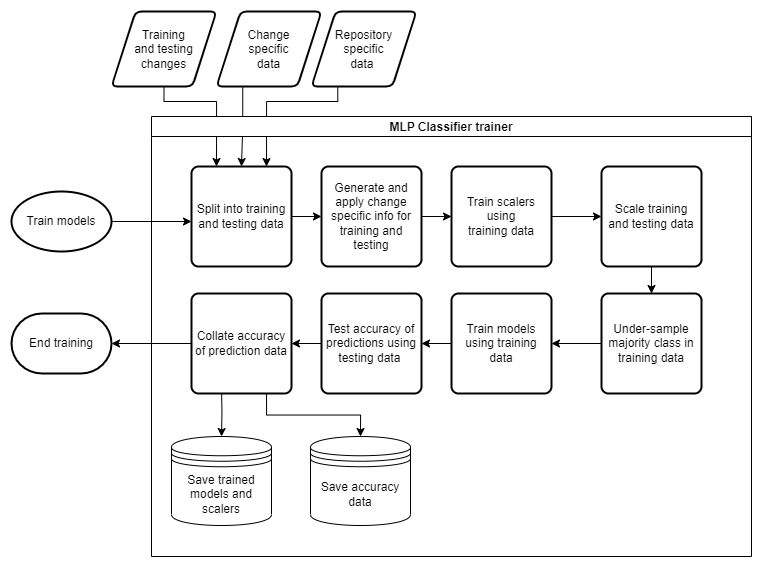
\includegraphics[scale=0.5]{images/neural-network-trainer-seperate.png}
    \caption{Flowchart describing the process used in the training of the neural network implementation.}
    \label{fig:neural-network-training-flowchart}
\end{figure}

The data box for the ``Training and testing changes'' in Figure~\ref{fig:neural-network-training-flowchart} represents the changes that are selected to train this model. This may be all the changes, changes for one repository, or changes with one status for one repository. As mentioned on page~\pageref{para:limited-to-ten-merged-changes} the time training and testing changes are selected from a time period chosen in the Algorithm~\ref{alg:data-collection-dataset} that still provides 10 merged changes for that repository. The data that is included for each change is detailed on page~\pageref{para:information-in-each-change-for-testing-data-set}.

The Repository specific data in this flowchart represents the data that is not unique to any one change. This is represented differently than in the Rule based recommender, as the data is collated into a pandas DataFrame that has the row labels as usernames and columns as data points. ``pandas'' is a Python library that allows easy analysis and manipulation of data\footnote{\url{https://pandas.pydata.org/}} and was used in this project to make handling the data much easier. Also unlike the rule recommender, any data that is collected for more than one time period is filtered so that the data kept is only that which is for the time period chosen by Algorithm~\ref{alg:data-collection-dataset}. Furthermore, whether a user can merge changes is added as a column unlike in the rule based recommender. This means that this data contains:
\begin{itemize}
    \item Code review vote counts from a specific time period
    \item Comment counts from a specific time period
    \item Whether a user can merge changes
\end{itemize}

Change-specific data represents data that is generated for each change but not stored in the training and testing data set. For this implementation, this is just the git-blame line counts generated by Algorithm~\ref{alg:git-blame-dataset}. Like the repository-specific data, this is filtered for the time period generated by Algorithm~\ref{alg:data-collection-dataset} for the repository the change is on.

This data is then split into testing and training data as detailed in the first process box. In the Python implementation sklearn's train\_test\_split\footnote{\url{\def\UrlBreaks{\do\/\do-\do.}https://scikit-learn.org/stable/modules/generated/sklearn.model_selection.train_test_split.html}. Accessed 12 May 2023.\def\UrlBreaks{\do\/\do-}} is used to appropriately split the changes.

Next, the change-specific information is added to the DataFrame for each change in turn. The data that is specific to each change is:
\begin{itemize}
    \item The git-blame line counts data filtered for the appropriate time period as generated by Algorithm~\ref{alg:git-blame-dataset}
    \item Whether the user voted on the change
    \item Whether the user approved the change
\end{itemize}

This is done in the Python implementation by making a deep copy of the pandas DataFrame for the change and then adding new columns for the git-blame data filtered for the associated time period.

Then the next section of the flowchart is the training of scalers using the training data. The trained scaler is then used to scale the training and testing data. This scaler is saved along with the model when the training completes because scaling the data is needed when the model is used to predict reviewers. Appropriately scaling data for neural networks helps improve the performance of the algorithms \citep{medium:importance-of-feature-scaling}. 

\label{para:training-when-scaling-caused-issues}When implementing this recommender system in Python the scaling of the data caused the produced recommendations to be not as expected. We tried removing the scaling of the data as a debugging step when training and this improved the accuracy of the model. Because the training and then evaluating the models take several days to complete, and this issue was noticed close to the deadline there was not enough time to find a solution that did not require disabling the scaling. As such for the training of the implementation that is analysed in Chapter~\ref{chap:evaluation} and discussed in Chapter~\ref{chap:conclusion}, the data was not scaled when training. However, as discussed by \cite{medium:importance-of-feature-scaling}, scaling should improve the model and not make it perform worse. Therefore, future work could include continuing to work on this implementation to fix this issue.

Next, the training data is under-sampled to reduce the bias given by the number of users in the pandas DataFrame that did not vote or approve the change. This is because the average change will have one or two code review votes. The method to under-sample in Python was by using imblearn's ClusterCentroids\footnote{\def\UrlBreaks{\do\/\do-\do.}\url{https://imbalanced-learn.org/stable/references/generated/imblearn.under\_sampling.ClusterCentroids.html\#imblearn.under\_sampling.ClusterCentroids}. Accessed 12 May 2023/\def\UrlBreaks{\do\/\do-}}. This library was proposed in \cite{JMLR:v18:16-365} and is built upon sklearn \citep[p. 1]{JMLR:v18:16-365}. Without under-sampling, the produced recommendations often recommended no one for a change.

The models are then trained using the training data. When training completes, the accuracy of the predictions the models make is tested using the training data. The model is asked to produce users who will vote or users who will approve depending on what the model was trained to do. Then this is compared to the users who actually approved or voted.

This testing process produces an accuracy score and confusion matrix. What these are and what they indicate is discussed further in Chapter~\ref{chap:evaluation} in the sections~\ref{section:accuracy-score} and \ref{section:confusion-matrix}.

\hspace{0.25cm}
\subsubsection{Producing recommendations}

Once the models are trained and saved, this implementation can just load the models and associated scalers to produce the recommendations. The process of this is shown in Figure~\ref{fig:neural-network-recommender-flowchart} by the use of a flow chart.

\begin{figure}[h]
    \centering
    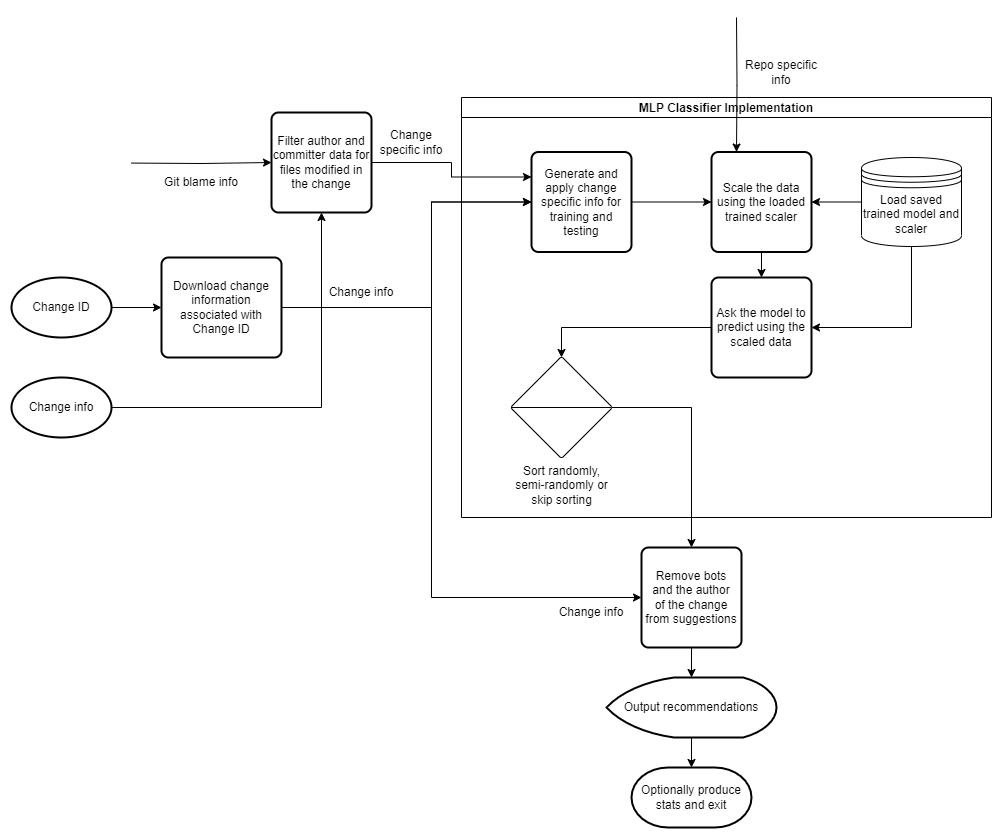
\includegraphics[scale=0.375]{images/neural-network-recommender-after-training.png}
    \caption{Flowchart describing the process used to produce recommendations on demand after training is complete.}
    \label{fig:neural-network-recommender-flowchart}
\end{figure}

The process can, similarly to the rule based recommender, take change info or a change ID. This is done using the same code in Python as for the rule based implementation.

The `approved' model produces a list of users who are predicted to approve the change and `voted' model produces a list of users who are predicted to vote on the change. Using these lists a third list of users who are predicted to have voted but not to have approved is made by performing a set difference operation on the lists. The list of users predicted to approve and the list of users predicted to vote but not approve are then used to make the recommendations.

While sklearn's MLP classifier implementation can produce probabilities associated with the user being in a particular class, this was not explored in this project as a way to rank the recommendations. \label{para:selection-mode-neural-network}Instead to order the recommendations one of three different techniques is used:
\begin{itemize}
    \item Random - The users predicted to vote or approve are randomly sorted to produce the recommendations list in order of strength
    \item Semi-random - The users predicted or vote or approve are randomly sorted but the distance they can move in the random sorting is limited to 5 positions from their start point.
    \item In-order - The users are recommended in the order they are in the input and predicted values lists.
\end{itemize}

The first two techniques are explored to evaluate whether not always prioritising the best reviewer would produce a noticeable difference in the accuracy of the recommendations. This is because the rule based recommender will produce the same list of users for a change in repositories and the list for the repository will be largely similar. Constantly recommending these users would overburden these users while leaving other good reviewers without being recommended. Being able to introduce some randomness would help alleviate this concern.

\label{para:mixing-approvers-and-voters}Furthermore, to avoid only recommending users who are predicted to approve users who are predicted to vote are mixed into a combined recommendations list after the ordering technique is applied. By default, this means that 3 users who are predicted to approve are present for every one user who is predicted to vote but not approve.

Using the models that were trained with no scaling for evaluation in Chapter~\ref{chap:evaluation} and discussion in Chapter~\ref{chap:conclusion}, the models produced no output if the input variables used to predict were not scaled using the scaler that was produced as part of Section~\ref{section:rule-based-implementation-training}. As mentioned on page~\ref{para:training-when-scaling-caused-issues} within that section, the removal of scaling data to address the very poor performance of the model is something that future work could look at and solve.